\section{RISMC Approach to PRA}
\label{sec:rismc}
The RISMC approach~\cite{RISMC} employs both deterministic and stochastic methods 
in a single analysis framework (see Figure~\ref{fig:RISMCoverview}). In the deterministic method 
set we include:
\begin{itemize}
  \item Modeling of the thermal-hydraulic behavior of the plant~\cite{BWR_SBO_Mandelli,BWRanalysis}
  \item Modeling of external events such as flooding~\cite{mandelliPSA2015}
  \item Modeling of the operators’ responses to the accident scenario~\cite{HRA_BoringReport2014}
\end{itemize}

\begin{figure}
    \centering
    \centerline{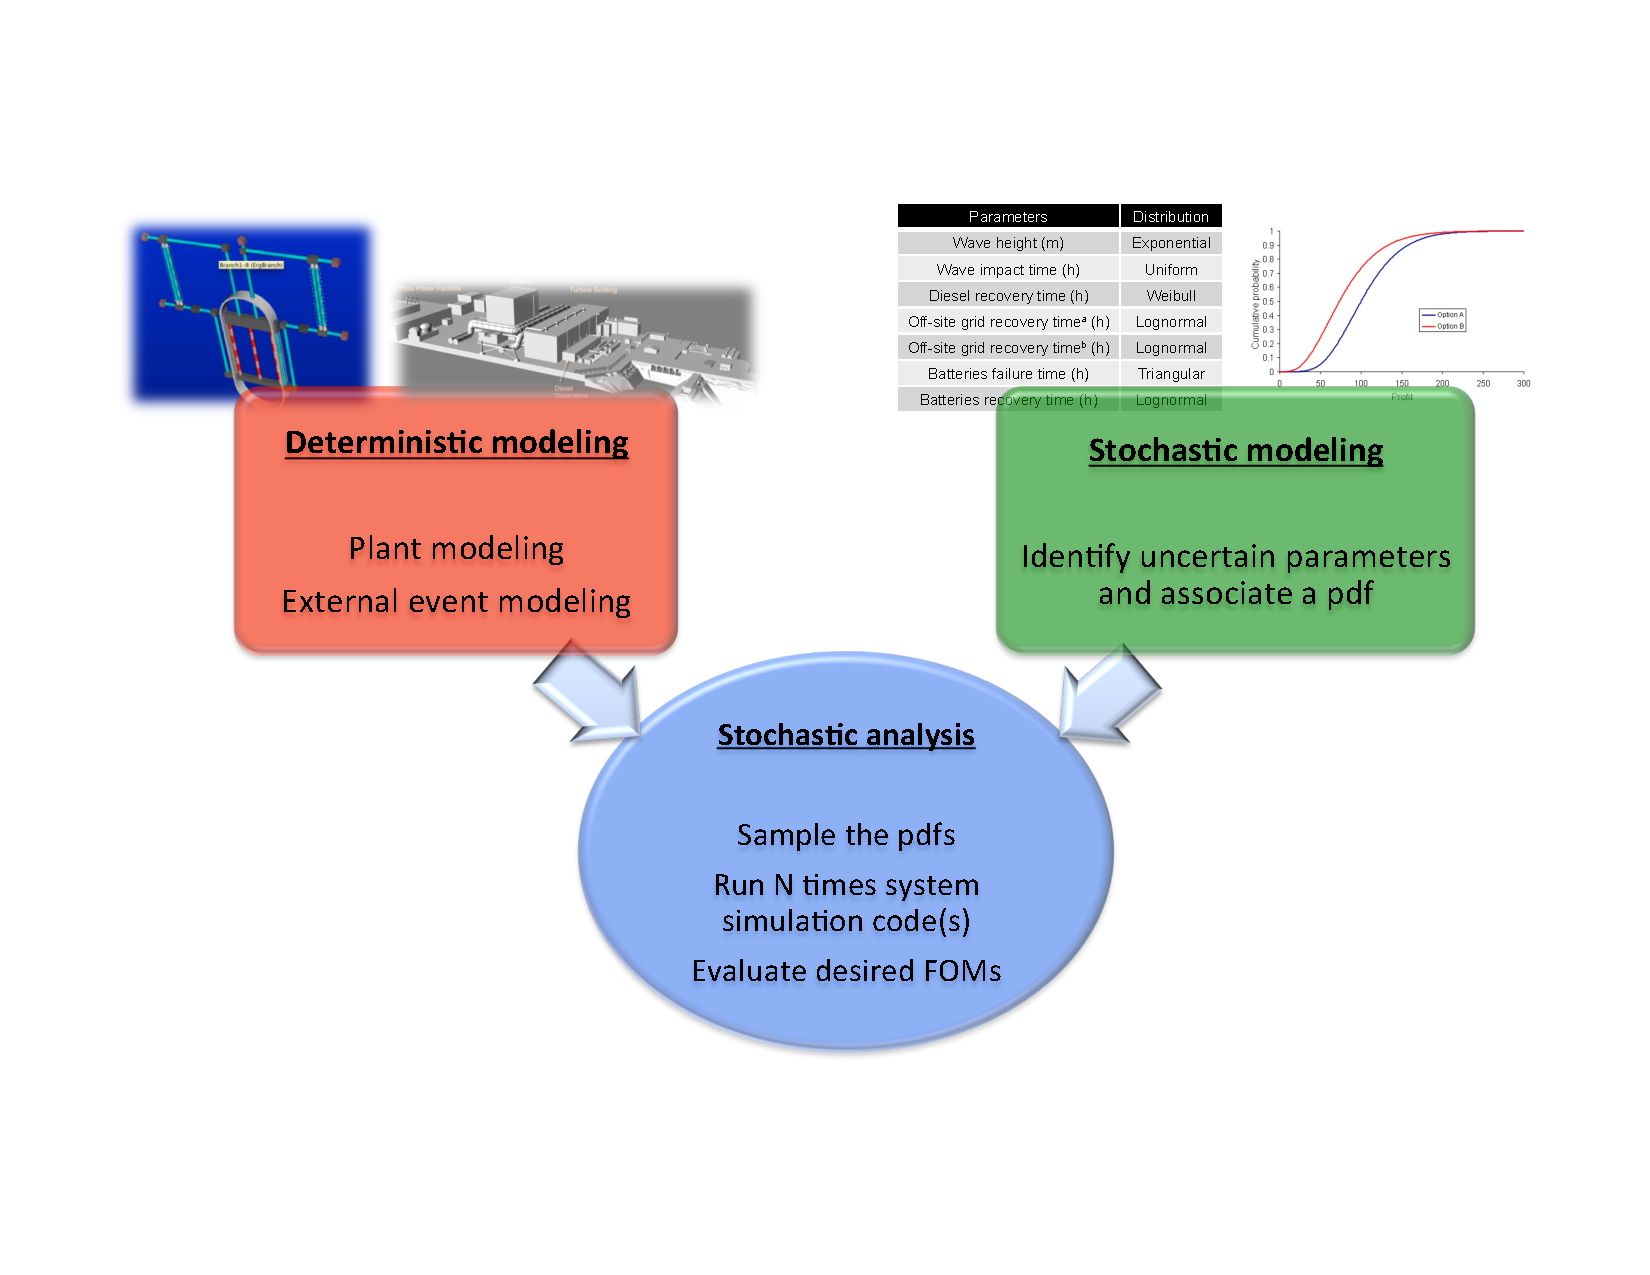
\includegraphics[scale=0.5]{RISMCoverview.pdf}}
    \caption{Overview of the RISMC approach}
    \label{fig:RISMCoverview}
\end{figure}

Note that deterministic modeling of plant or external events can be performed by employing 
specific simulator codes but also surrogate models, known as Reduced Order Models (ROMs)~\cite{ROM_Khalik}. 
ROMs would be employed in order to decrease the high computational costs of employed codes.
In addition, multi-fidelity codes can be employed to model the same system; the idea is to 
switch from low-fidelity to high-fidelity code when higher accuracy is needed (e.g., use 
low-fidelity codes for steady-state conditions and high-fidelity code for transient conditions).

\subsection{System Modeling}

Modeling of the actual plant is performed using system analysis codes which simulate the temporal 
evolution of the plant given the sampled timing/sequencing of events. Example of codes employed 
in the nuclear industry are RELAP5-3D~\cite{relap5} and MELCOR~\cite{Melcor}. 
Example of RISMC analysis performed using the RISMC approach can be 
found in~\cite{BWR_SBO_Mandelli,BWRanalysis,PRA_comparison_PSA2015}.

\subsection{Human Modeling}

\subsection{External Event Modeling}
Modeling of external events (e.g., seismic or flooding) follows the same philosophy behind the RISMC
approach: model the phenomena from both a deterministic (i.e., by employing codes) and stochastic 
point of view (i.e., by introducing stochastic elements into the simulation). This approach have the 
relevant advantage that the external event can interact directly with the plant simulation. 
This interaction can occur not only at the beginning at the beginning of the accident scenario but also
during the accident scenario itself. Thus, the external event is not only considered as initial condition
imposed at the beginning of the analysis but is a boundary condition that evolve in time along with the
actual plant simulation.

\subsection{ROM Modeling}
Each RISMC analysis often requires a large amount of samples; this is due to the fact that the 
number of stochastic parameters is very large and the uncertainties may be significant. 
The scope of the analysis is not only to determine outcome variables such as core damage probability 
but, more in general, evaluate the system response for different combinations of the stochastic
parameters in order to determine specific observable outcomes (e.g., plant damage). In addition, 
a single evaluation of the system response in Step 2 is often computationally expensive. 
This is often the case when multi-physics simulator codes and/or multiple codes are employed in an 
integrated simulation run.

These two issues, large number of samples required and computational cost of each simulation run, 
make it challenging to perform a full PRA analysis of complex systems such as nuclear power plants.  
In order to overcome this challenge, two possible solutions are available: reduce the required 
number of samples or reduce the computational cost of each simulation run.

Both solutions rely on the development of ROMs~\cite{ROM_Khalik}, also known as surrogate models. 
ROMs are mathematical models that infer the structure of a given set of data points using a
blend of regression and interpolation techniques. In Solution 1, ROMs are built in order to generate 
the minimum set of samples that allows to determine the outcome variables: this is called smart or 
adaptive sampling. On the other hand, Solution 2 aims to build a ROM as a substitute of the simulation 
code itself (i.e., a surrogate for a complex calculation).  ROMs are in fact much quicker to run 
(a single ROM evaluation is on the order of $ms$) but, ROMs only approximate the simulation code and 
thus an intrinsic uncertainty is always present.

\subsection{System Stochastic Modeling}
In the RISMC stochastic modeling we include all steps required to include in the analysis the 
stochastic parameters that are of interest in the analysis such as: uncertain parameters and stochastic 
failure of system/components.
This is performed by employing stochastic analysis tools (e.g., RAVEN~\cite{RAVEN_PSAM_2014}) that are 
interfaced with the chosen system analysis codes. This interface is responsible to:

\begin{enumerate}
  \item perturb the input file of the system analysis code by inserting in it the values sampled by the
        stochastic analysis tools
  \item execute the simulation run given the input file generated in Step 1
  \item collect the output of the simulation run so that a link between sampled input values and simulation 
        outcome is created      
\end{enumerate}

